%
%  outline latex source document for AV assignment 1.
%  use pdflatex to format this.
%
\documentclass[10pt,a4paper,oneclumn]{article}
\usepackage{amssymb,amsmath}            % if some maths is needed
\usepackage{graphicx}                   % if any images are to be included
% pick a different font if desired
\usepackage{times}

\title{Advanced Vision Assignment 2 Report}  % AILP: please use this title.
\author{Mindaugas Dabulskis, Marat Subkhankulov}                      % replace with name or exam number
\date{26th February 2013}                 % replace with actual date

\begin{document}

\maketitle  % insert title, author info
%

\section{Final Touch}

\begin{figure}[h!]
\centering
  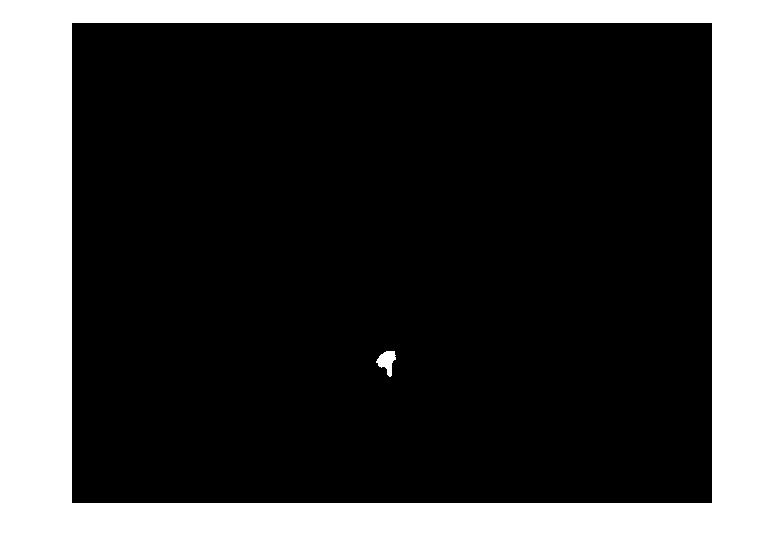
\includegraphics[width=5cm]{cleanedYell.jpg}
  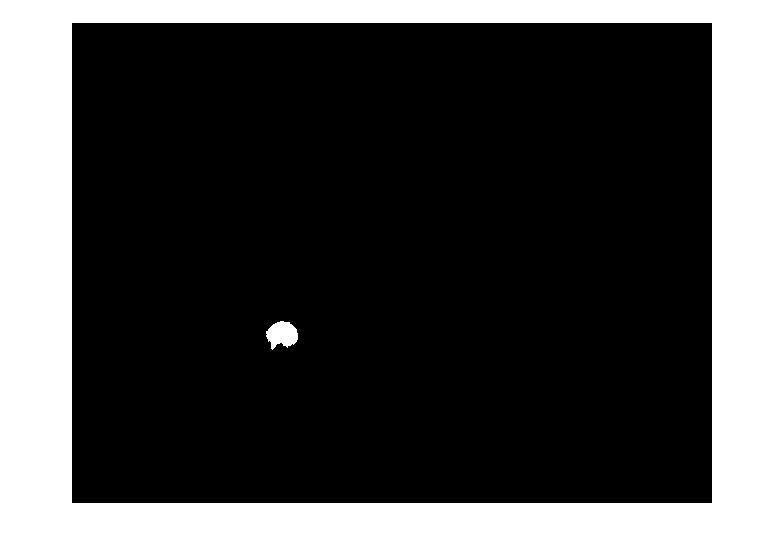
\includegraphics[width=5cm]{cleanGreen.jpg}
  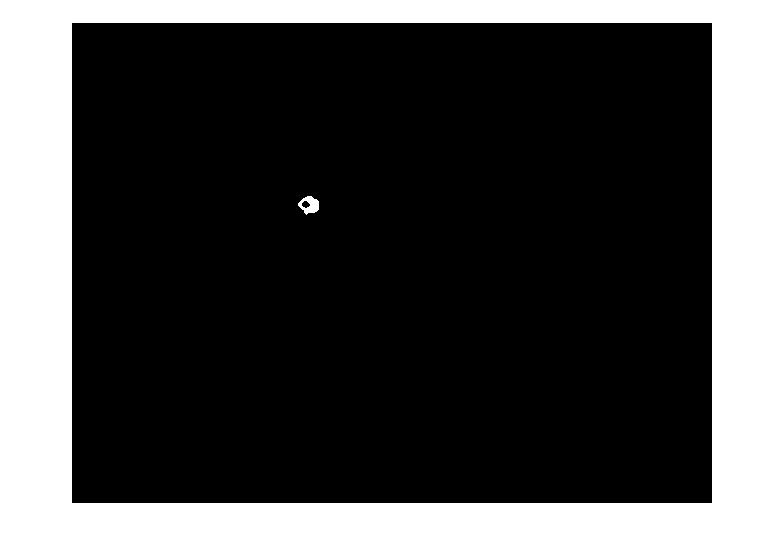
\includegraphics[width=5cm]{cleanRed.jpg}
  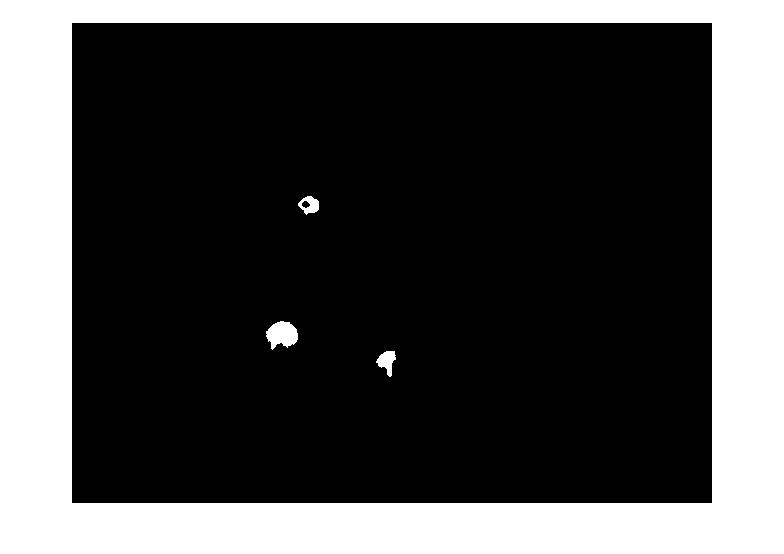
\includegraphics[width=5cm]{cleanAll.jpg}
\caption{Cleaned images}
\end{figure}

Final clean up and ball identification was made using matlab \textbf{bwlabel} and \textbf{regionprops} functions. The function \textbf{bwlabel} takes our intermediate file, which we got after applying all the masks, and labels all the connected objects in the file. Later, this file is supplied to \textbf{regionprops} function, which measures and returns set of the properties for each connected object in the file. We only needed three properties:

\begin{enumerate}
\item \emph{Area} - number of actual pixels in the region,
\item \emph{PixelIdxList} - vector containing the linear indices of the pixels in region,
\item \emph{PixelList} - matrix specifying the locations of pixels in the region.
\end{enumerate}

The idea was: 
\begin{enumerate}
\item to find maximum connected object in the file by the pixels area, 
\item set all other connected object areas pixel to 0 (delete these areas), 
\item find the middle point of the largest connected objects area. 
\end{enumerate}

Second point cleaned the image of all the noise, because the object with biggest area was the ball itself. Third point was needed for evaluation, to evaluate how much our detected ball differs from ground truth. We had four different approaches how to calculate the mass of the ball:

\begin{enumerate}
\item Use the mean of the area pixels,
\item use the median of the area pixels,
\item use the maximum and minimum pixels in \textbf{y} and \textbf{x} coordinates and find the mean between them. This creates a bounding box of the area and finds it centre.
\end{enumerate}

The evaluation of these approaches are reported in the section below. We decided to use just normal mean, but left an option to change if needed and found that other approaches with different data sets works better. We stored all found centres in the matrix. The format of that matrix is exactly the same as the format for the ground truth. In next stage we just plot the found mass centres on each image with the centre from ground truth and draw the trajectory at the end by connecting all the points.

\section{Experiments and results}

\begin{figure}[h!]
\centering
  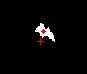
\includegraphics{errorCroped.jpg}
\caption{Image in which the distance between ground truth (+) and found mass centre (.) is bigger than 10 pixels}
\end{figure}

\begin{figure}[h!]
\centering
  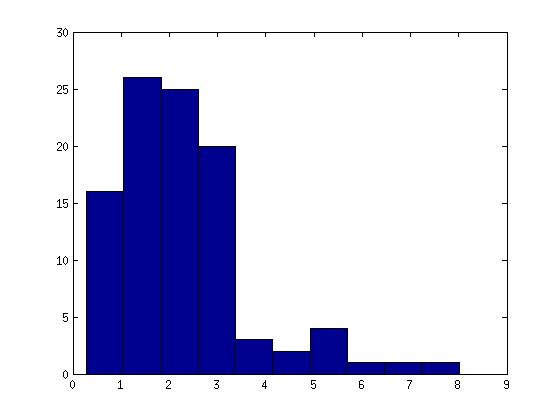
\includegraphics[width=3cm]{redHist.jpg}
  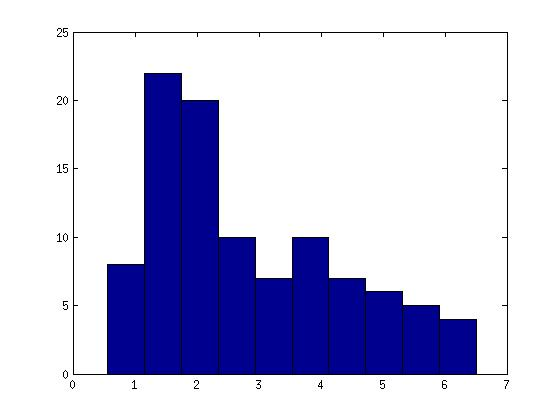
\includegraphics[width=3cm]{greenHist.jpg}
  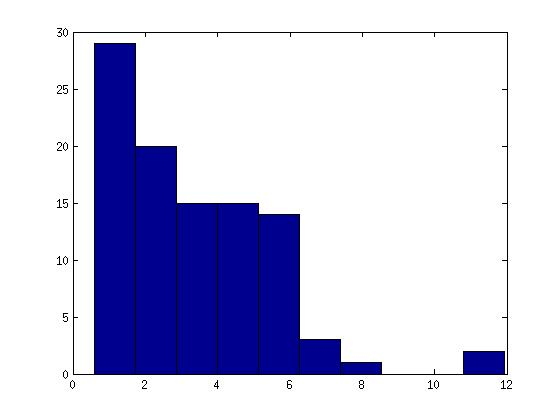
\includegraphics[width=3cm]{yellowHist.jpg}
\caption{Cleaned images}
\end{figure}

\begin{figure}[h!]
\centering
  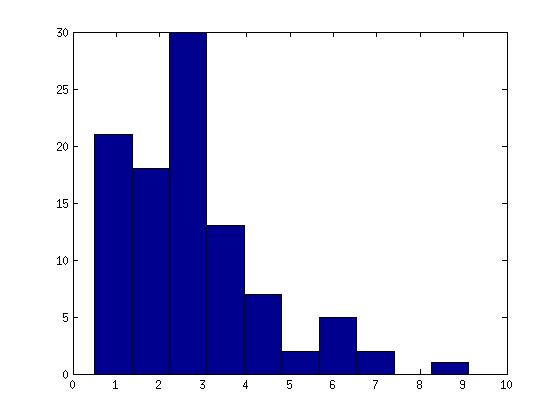
\includegraphics[width=3cm]{redHistBound.jpg}
  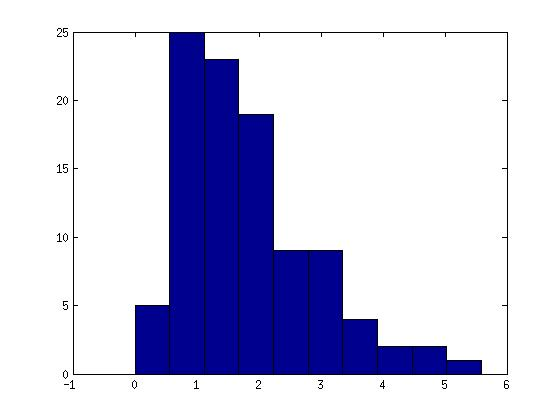
\includegraphics[width=3cm]{greenHistBound.jpg}
  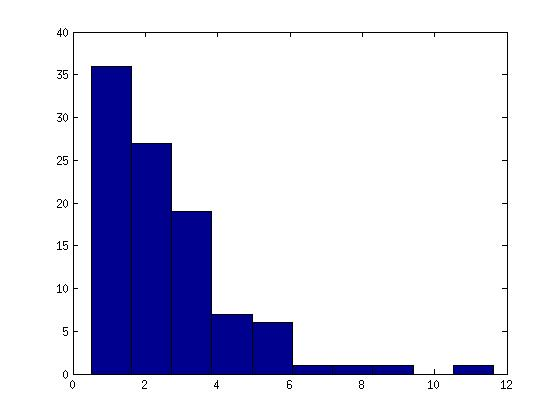
\includegraphics[width=3cm]{yellowHistBound.jpg}
\caption{Cleaned images}
\end{figure}

\begin{figure}[h!]
\centering
  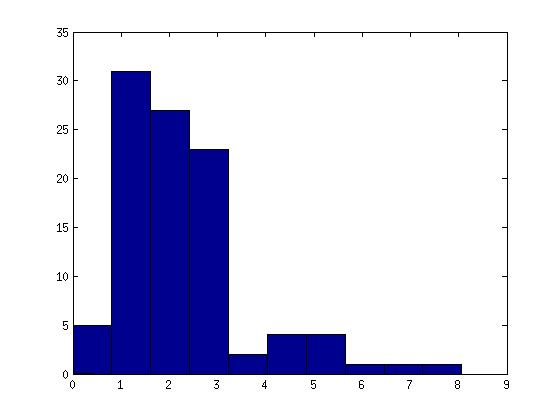
\includegraphics[width=3cm]{redHistMedian.jpg}
  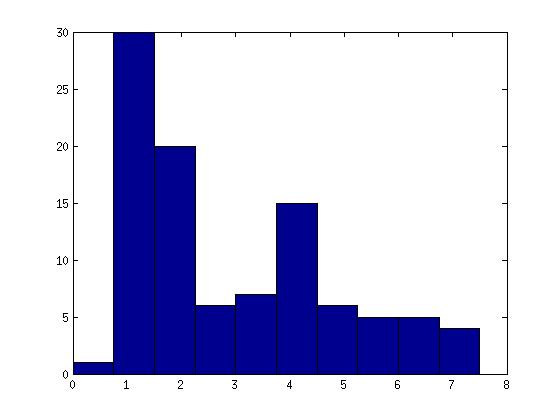
\includegraphics[width=3cm]{greenHistMedian.jpg}
  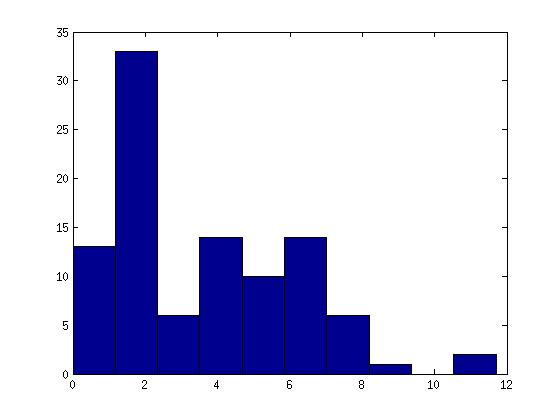
\includegraphics[width=3cm]{yellowHistMedian.jpg}
\caption{Cleaned images}
\end{figure}

\begin{figure}[h!]
\centering
  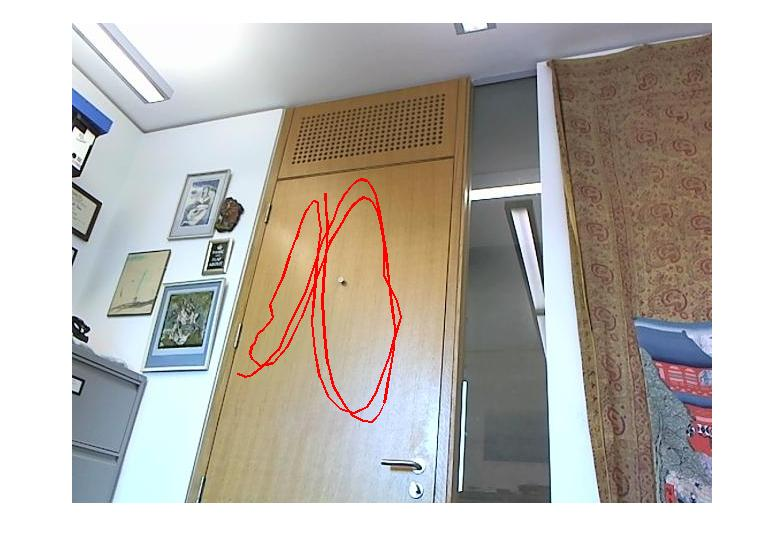
\includegraphics[width=3cm]{redMean.jpg}
  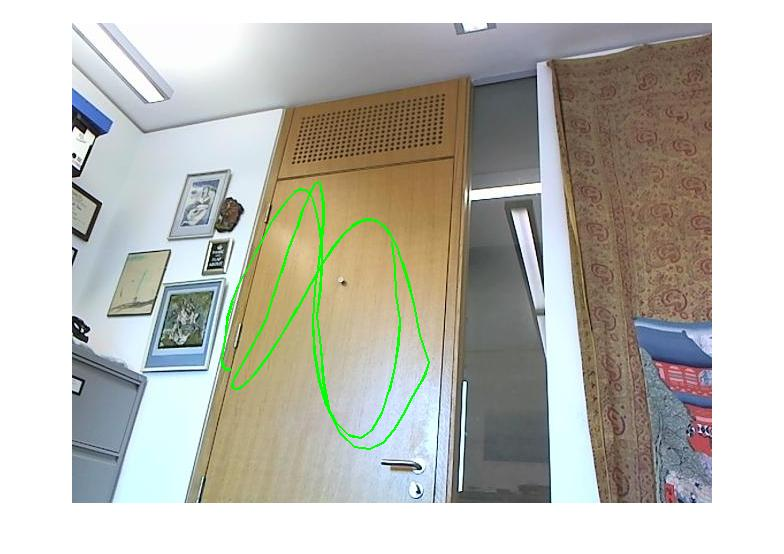
\includegraphics[width=3cm]{greenMean.jpg}
  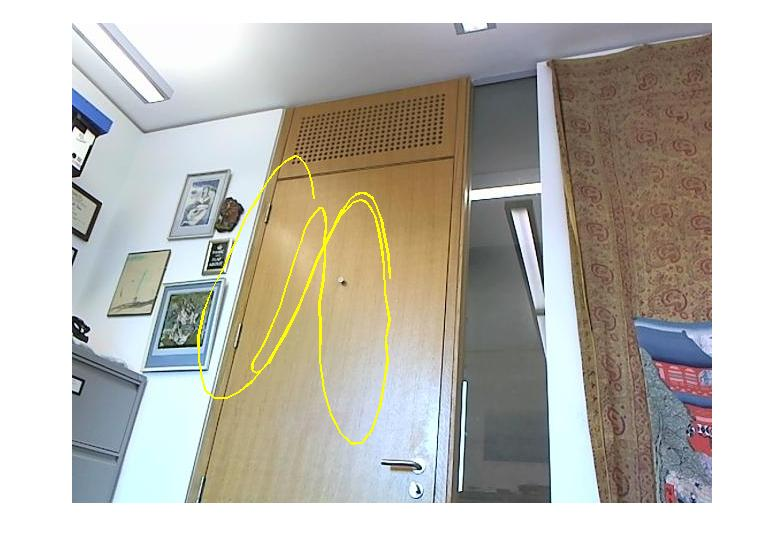
\includegraphics[width=3cm]{yellowMean.jpg}
\caption{Cleaned images}
\end{figure}

\begin{figure}[h!]
\centering
  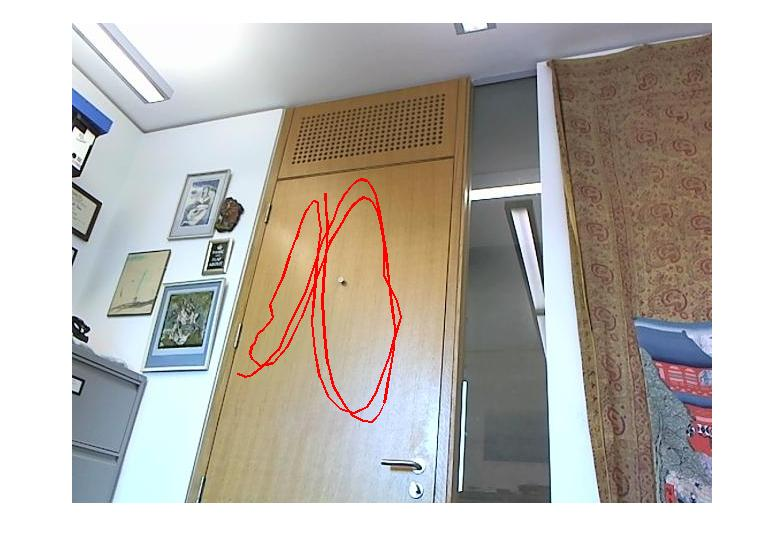
\includegraphics[width=3cm]{redMean.jpg}
  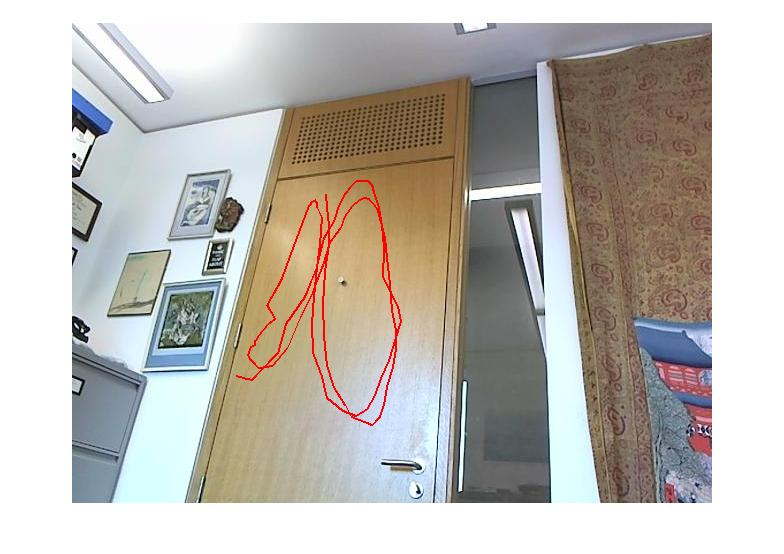
\includegraphics[width=3cm]{redBound.jpg}
  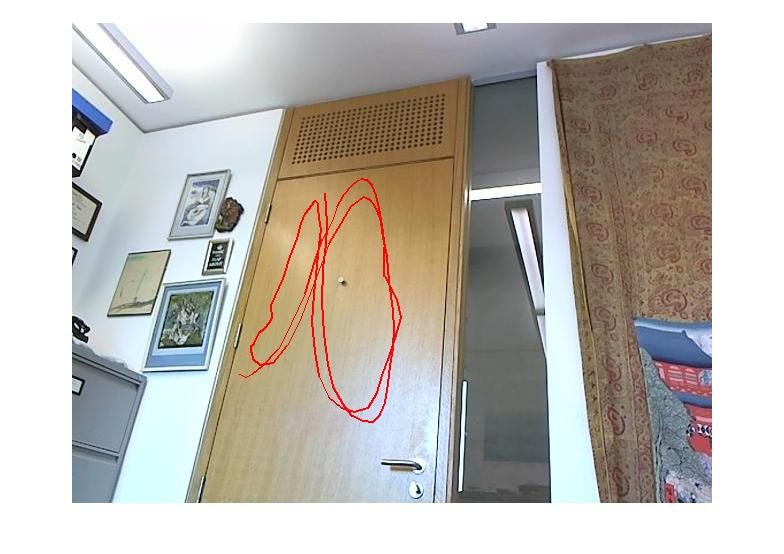
\includegraphics[width=3cm]{medianRedTrack.jpg}
\caption{Cleaned images}
\end{figure}

The experments shows that in all the image balls were detected. However, using the criterion that the detected ball mass centre should be more futher than 10 pixels, we found out that in two images it is not the case. The main reason while the centre is futher is because of the junglers fingers. The fingers cover half the ball, thus it is not even hard to recognise the ball, but also imposible to get whole ball, because it is partly covered. Automaticly, we only detec half the ball, resulting in shifted mass centre. Potiancial remedies would be somehow identify that the ball is in junglers hand and make bigger bounding box for the ball at those points. This way we would increase the area of the ball artificialy, which would be more similar to actual ball size than what is recognised.

We have aso evaluated diffrent aproches to the mass centre calculation. From statistics we can see that bounding box aproch has the smaller total error and have only one image in which found mass centre in yellow ball is futher than 10 pixels, compared to other aproches, which have two images. This is a case, because in this aproch we take account that half the ball might be covored by hand, thus we creating artificial area in which we predict that the ball is located. If we look into individual balls error, we would noticed that with bounding box approch red ball has the largest error compared with other aproches. This is because red ball has very distinguiched color and it is very easy to recognise, thus usually the ball is easily recognised. That is why in mean and median approch the red balls error is smallest. However, in bounding aproch we creating artificial area, which might not be correct area of the ball, thus we make more mistakes. Inconclusion, bounding box approch works great n balls, which can be hard to recognise, but does not work well with easily recognisable balls. We decided not to use bounding box approch, because the drawn path is quite chopy and not as smooth as other two approches.

\begin{table} [t,h]
\caption{\label{table1} \textit{Mean}}
\vspace{2mm}
\centerline{
\begin{tabular}{|c|c|c|c|}
\hline
 & Red & Green & Yellow \\
\hline  \hline
ball found in images & 98/98 & 98/98 & 98/98 \\
\hline
mass centre is less than 10 pixels from ground truth & 98/98 & 98/98 & 96/98 \\
\hline
maximum error & 8.0093 &6.5060 &  11.9423 \\
\hline
minimum error & 0.2799 &  0.5622 &  0.5995 \\ 
\hline
one ball error & 224.0428 &   276.9718 & 328.6480 \\
\hline
total error & \multicolumn{3}{|c|}{829.6625} \\
\hline
\end{tabular}}
\end{table}

\begin{table} [t,h]
\caption{\label{table1} \textit{Bound}}
\vspace{2mm}
\centerline{
\begin{tabular}{|c|c|c|c|}
\hline
 & Red & Green & Yellow \\
\hline  \hline
ball found in images & 98/98 & 98/98 & 98/98 \\
\hline
mass centre is less than 10 pixels from ground truth & 98/98 & 98/98 & 97/98 \\
\hline
maximum error & 9.1241 &  5.5902&  11.6297 \\
\hline
minimum error &0.5000 20 & 0 & 0.5000\\ 
\hline
one ball error & 264.7848 &  189.4427 & 258.1291 \\
\hline
total error & \multicolumn{3}{|c|}{712.3566} \\
\hline
\end{tabular}}
\end{table}

\begin{table} [t,h]
\caption{\label{table1} \textit{Median}}
\vspace{2mm}
\centerline{
\begin{tabular}{|c|c|c|c|}
\hline
 & Red & Green & Yellow \\
\hline  \hline
ball found in images & 98/98 & 98/98 & 98/98 \\
\hline
mass centre is less than 10 pixels from ground truth & 98/98 & 98/98 & 96/98 \\
\hline
maximum error & 8.0623 & 7.5000 & 11.7047 \\
\hline
minimum error & 0 & 0 & 0 \\ 
\hline
one ball error & 227.6602 &   298.2528 & 363.9370 \\
\hline
total error & \multicolumn{3}{|c|}{889.8500} \\
\hline
\end{tabular}}
\end{table}

\subsection{References}

References should be numbered in order of appearance, 
for example \cite{ES1}, \cite{ES2}, and \cite{ES3}. 
You \emph{can} use \texttt{bibtex} to prepare references,
or do it by hand if there are very few.

%
\bibliographystyle{IEEEtran}
\begin{thebibliography}{10}
\bibitem[1]{ES1} Smith, J. O. and Abel, J. S., 
``Bark and {ERB} Bilinear Transforms'', 
IEEE Trans. Speech and Audio Proc., 7(6):697--708, 1999.  
\bibitem[2]{ES2} Lee, K.-F., Automatic Speech Recognition: 
The Development of the 
SPHINX SYSTEM, Kluwer Academic Publishers, Boston, 1989.
\bibitem[3]{ES3} Rudnicky, A. I., Polifroni, Thayer, E. H.,
 and Brennan, R. A.  
"Interactive problem solving with speech", J. Acoust. Soc. Amer., 
Vol. 84, 1988, p S213(A).
\end{thebibliography}
\end{document}
